\scanpage{82}
\margin{81}
ou de façon équivalente, par les $g^\alpha_{x,y}$ \inserted{$\in\unsure{\widehat\Pi_\alpha|\widehat\pi_\alpha}$}, où $\alpha\in A$, $x,y\in I_\alpha$ (cf plus haut). Ceci rappelé, on peut espérer donner des ``formules'' explicites, \uline{dépendant bien sûr des propriétés arithmétiques précises du point particulier} $x$, et \uline{caractéristiques de} $x$ (dans la situation Mordell-Weil-Néron), qui donnent $f_l(u)$ \uline{en termes} des paramètres précédents fixant $u$. C'est là un travail fascinant en perspective, que je n'ai pratiquement pas amorcé encore pour le moment!
\margin{\figure{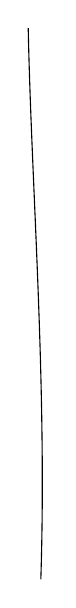
\begin{tikzpicture}\draw (0,0)..controls(.08,2.5)and(-.12,5)..(-.16,7);\end{tikzpicture}}}

À vrai dire, la démonstration via Mordell-Weil de l'unicité d'un $x$ \inserted{$\in X_K$} \unsure{qui} correspond à une classe donnée dans $H^1(\Gamma,\widehat\Pi_1(x_0))$, montre qu'on a unicité $=$ si on \deleted{\unsure{en donne}} \inserted{connaît} seulement l'élément correspondant à \deleted{\unsure{un}}
\[
\tag{34}(f_{x_0,x})_{\mathrm{ab}}\in H^1(\Gamma,\widehat\Pi_1(X,x_0)_{\mathrm{ab}}),
\]
et on peut déjà essayer de déterminer, par ``formules explicites'', les $(f_l)_{\mathrm{ab}}$ correspondant à des chemins $x_0\longrightarrow x$. On est réduit à regarder la $=$ question en remplaçant $X$ par une VA ou ext. d'icelle,

\margin{(C'est une question particulière, qui \unsure{bien plus intéressante|en plus intéressante} \illegible{2} \unsure{un problème} \unsure{variable} \unsure{en} $X$ \unsure{au-dessus de} $\unsure{\mathbb Q}$ \illegible{2}.)}
